\chapter{Modeling}
Ai fini della classificazione, si è scelto di usare l'algoritmo \textbf{C4.5}, in particolare nella versione implementata da Weka, \textbf{J48}.

\section{Tecnica di modeling}
C4.5 è un algoritmo usato per generare alberi di decisione sviluppato da \texttt{Ross Quinlan} ed è un'estensione del precedente ID3. Nel corso degli anni esso è stato soppiantato da una sua evoluzione, C5.0, distribuito commercialmente da Quinlan di cui però è disponibile una versione \textit{free} \textit{mono-threaded} sotto licenza GPL\cite{C50}.


\subsection{Descrizione di C4.5}
L'albero costruito da C4.5 presenta le seguenti caratteristiche:
\begin{itemize}
	\item Ogni nodo interno eseguono un test su un attributo.
	\item Ogni ramo corrisponde ad un valore dell'attributo.
	\item Ogni foglia costituisce una classe.
\end{itemize}

I nodi interni dell'albero eseguono un test su un attribuuto, 

Il criterio per valutare quale attributo classifica meglio i dati è l'\textbf{entropia}. Si consideri:
\begin{itemize}
	\item $S$ il training set.
	\item $C_j$ un'etichetta di classe in $C_1, C_2, ..., C_k$.
	\item $FR(C_i, S)$ con $1 \leq i \leq k$ le frequenze relative delle instanze in $S$ che appartengono alla classe $C_i$.
\end{itemize}
L'entropia $E$ su $S$ è calcolata come:
$$ E(S) = - \sum_{i=1}^{k} FR(C_i, S)log(FR(C_i, S)) $$
e misura l'\textbf{incertezza} contenuta in $S$

Nel caso in cui le classi siano due, positive e negative, l'entropia si calcola come:
$$ E(S) = -plog_2p - nlog_2n $$
dove $p$ rappresenta le istanze positive e $n$ quelle negative.

L'\textbf{Information Gain} $G(S,t)$ rappresenta quanto diminuisce l'entropia con la distribuzione delle istanze in $S$ in base al test $t$.

Si considerino $S_1, ..., S_z$ le partizioni di $S$ da parte di un test $t$ su un attributo $A_i$:
$$ G(S,t) = E(S) - \sum_{i} \frac{|S_i|}{|S|}E(S_i) $$
Il criterio di information gain sceglie il test $t$ che massimizza $G(S,t)$.

Il difetto di quest'ultimo è il favorimento di test con molti valori distinti. Una soluzione potrebbe essere quella di utilizzare solo test binari, ma ciò porterebbe ad una perdita maggiore di interpretabilità del modello e ad un incremento del costo computazionale. Un'altra soluzione potrebbe essere quella di pesare l'information gain rapportandola alla quantità di infomazione potenziale della partizione $P(S,t)$ senza considerare la classe, che si calcola come:
$$ P(S,t) = -\sum_{i} \frac{|S_i|}{|S|}log(\frac{|S_i|}{|S|}) $$

Successivamente scegliamo il test $t$ che massimizza $G(S,t)/P(S,t)$. Questa quantità viene chiamata \textbf{gain ratio}.

Lo pseudo-codice di C4.5 è:
\begin{algorithm}[!htb]
	\caption{C4.5($Esempi, AttributoTarget, Attributi$)}
	\begin{algorithmic}[1]
		\State Crea un nodo radice $Root$ dell'albero
		\If{tutti gli $Esempi$ sono di classe $C_i$}
			\State \Return il singolo nodo $Root$ con etichetta = valore più comune di
			\State$AttributoTarget$ in $Esempi$
		\Else
			\State $A \gets$ l'attributo da $Attributi$ che meglio classifica $Esempi$ (gain ratio
			\State o information gain più alto)
			\State L'attributo di decisione per $Root \gets A$
			\ForAll{valore $v_i$ di $A$}
				\State Aggiungi un nuovo ramo sotto $Root$, che corrisponde al test $A=v_i$
				\State Sia $Esempi(v_i)$ il sottoinsieme di $Esempi$ che ha il valore $v_i$ per
				\State $A$
				\If{$Esempi(v_i)$ è vuoto}
					\State Aggiungi sotto questo ramo un nodo foglia con etichetta =
					\State valore più comune di $AttributoTarget$ in $Esempi$
				\Else
					\State C4.5($Esempi(v_i), AttributoTarget, Attributi - {A}$)
				\EndIf
			\EndFor
		\EndIf
	\end{algorithmic}
\end{algorithm}

\pagebreak

\subsection{Pruning}
Gli alberi di decisione pienamente sviluppati spesso lamentano una struttura che contiene componenti non necessarie; in linea generale si consiglia di semplificarli prima di distribuirli: questa operazione di semplificazione si chiama \textit{pruning} (potatura).
Quando si costruisce l'albero completo e lo si pota in un secondo momento, si adotta una strategia di \textit{postpruning}, piuttosto che di \textit{prepruning}. Quest'ultimo si occupa di decidere durante la costruzione dell'albero quando smettere di sviluppare sottoalberi. Il postpruning sembra offrire qualche vantaggio, per esempio in situazioni in cui due attributi presi singolarmente non sembrino contribuire molto ma acquisiscono un potere predittivo maggiore quando combinati. 

Due approcci di postpruning sono il \textit{subtree replacement} e il \textit{subtree raising}. L'idea del subtree replacement è selezionare qualche sottoalbero e sostituirlo con singole foglie. Il secondo approccio, il subtree raising, è più complesso, ed è quello implementato da C4.5, nella fattispecie dal suo gemello J48\cite{Witten:2011:DMP:1972514}. Si consideri l'albero in \ref{fig:subtree}(a) che, dopo la potatura, diventa \ref{fig:subtree}(b). L'intero sottoalbero da C in giù è stato "innalzato" per sostituire il sottoalbero B. Si noti che, nonostante nell'immagine i figli di B e C sono foglie, essi possono essere a loro volta sottoalberi. Ovviamente, dopo aver eseguito questa operazione di ascesa, è necessario riclassificare gli esempi ai nodi 4 e 5 nel nuovo sottoalbero innestato in C. Questo è il perché i figli di C sono diventati 1', 2' e 3', per indicare che non sono gli stessi nodi di prima ma differiscono per l'inclusione degli esempi precedentemente coperti da 4 e 5.
Il subtree raising è un'operazione potenzialmente \textit{time-consuming}. Nelle implementazioni reali in genere ci si limita ad innalzare il sottoalbero del ramo più popolare. Cioè, si fa quello fatto in \ref{fig:subtree} purché il ramo da B a C abbia più esempi di training rispetto ai rami da B a 4 o da B a 5. Altrimenti, se per esempio il nodo 4 avesse più istanze di training in assoluto, si dovrebbe innalzare il nodo 4 per sostituire B e riclassificare tutti gli esempi sotto C e 5 nel nuovo nodo.
\begin{figure}[!hbtp]
	\centering
	\includegraphics[width=\textwidth,height=\textheight,keepaspectratio]{./images/subtree_raising}
	\caption{Esempio di subtree raising}
	\label{fig:subtree}
\end{figure}

\section{Rappresentazione del modello}
%\input{./images/tree3.tex}
%\begin{figure}[!htbp]
%	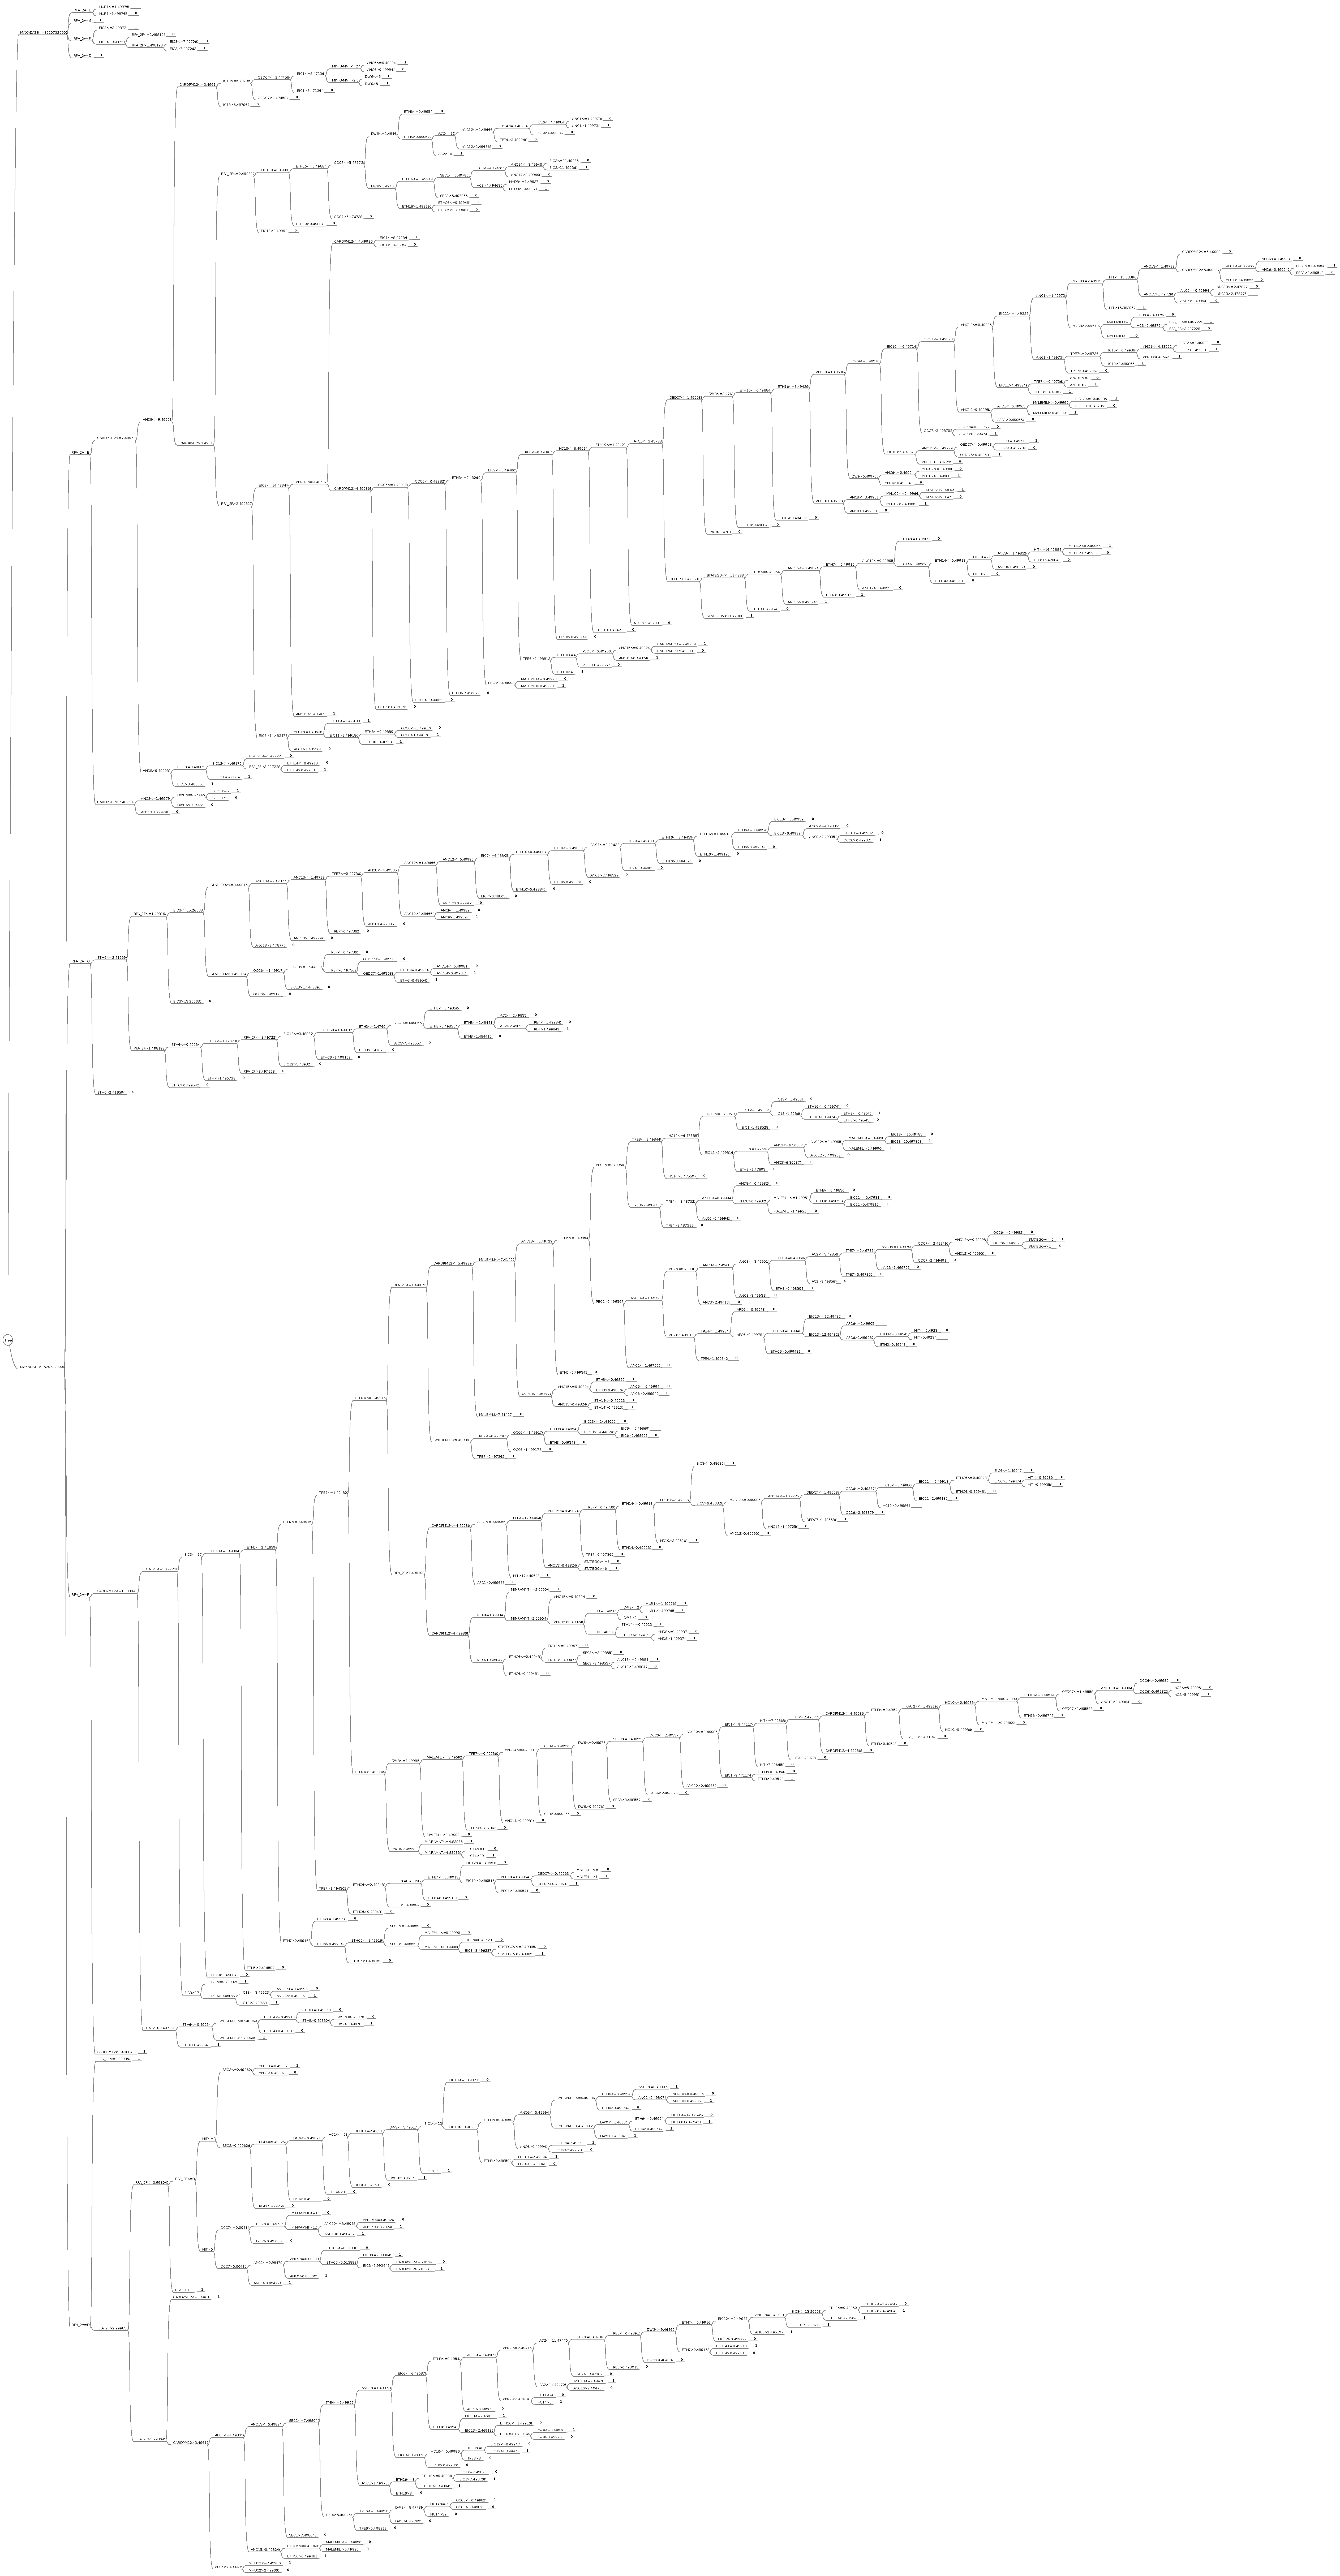
\includegraphics[width=\textwidth,height=\textheight,keepaspectratio]{./images/tree}
%	\caption{Modello}
%	\label{fig:tree}
%\end{figure}
%
%\pagebreak

\section{Costruzione del modello}

\section{Valutazione del modello}